\subsection{Research Gaps}
\label{sec:research_gaps}

\begin{figure*}[pos=htbp]
  \centering
  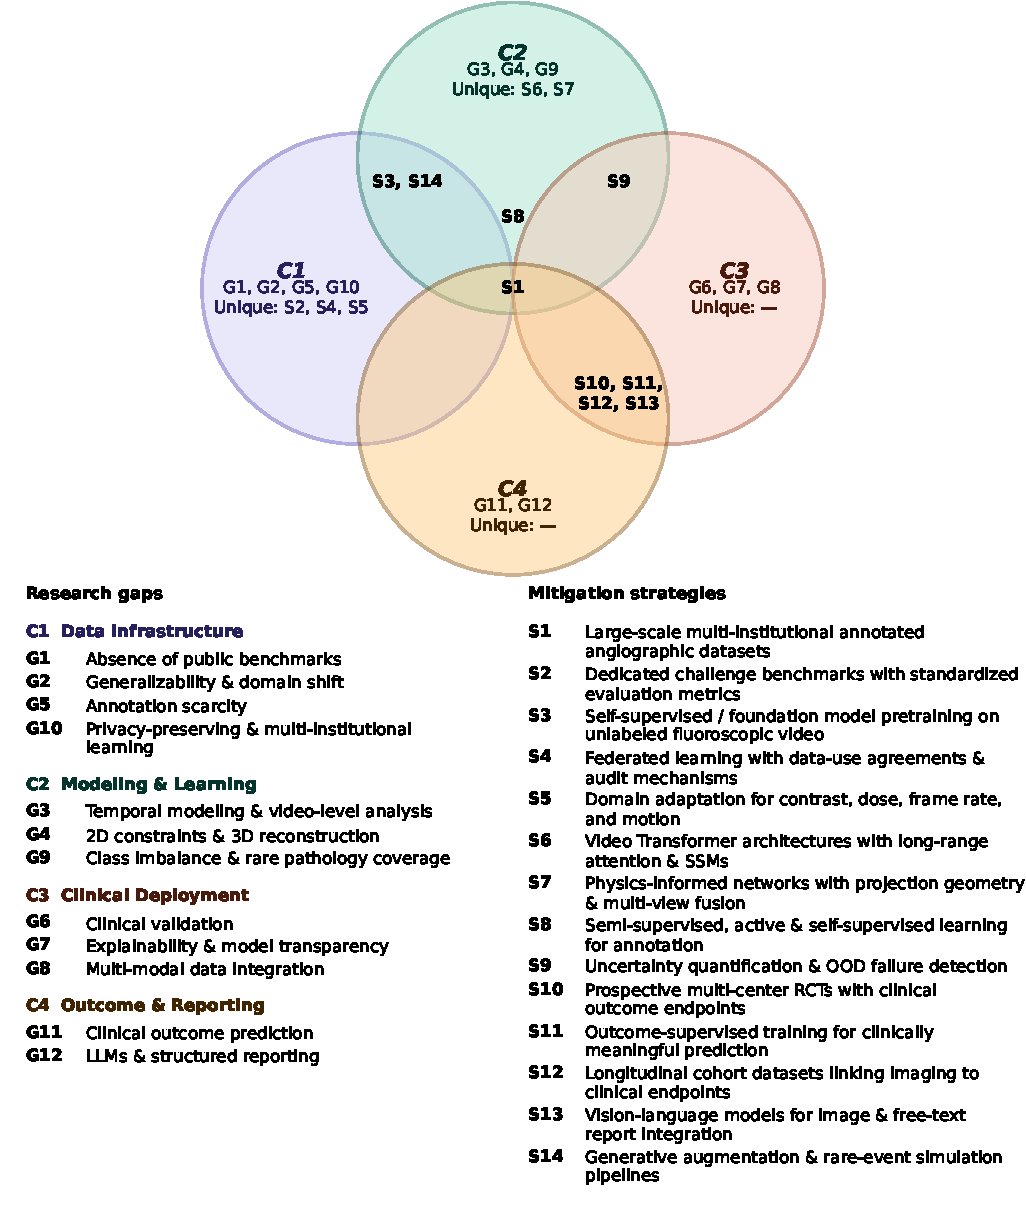
\includegraphics[width=0.9\textwidth]{figs/venn_diagram.pdf}
  \caption{Research gaps grouped into four clusters, with mitigation strategies. C1: Data Infrastructure (G1, G2, G5, G10); C2: Modeling \& Learning (G3, G4, G9); C3: Clinical Deployment (G6, G7, G8); C4: Outcome \& Reporting (G11, G12). Strategy codes (S1--S14, defined in the legend) sit in the clusters or overlaps they serve; \edit{unlabeled} overlaps have no shared strategy. Gap codes follow Table~\ref{tab:research_gaps}.}
  \label{fig:venn_gaps}
\end{figure*}

We identified twelve research gaps (G1--G12) and organized them into four clusters (C1--C4), which are shown in Figure~\ref{fig:venn_gaps}. \textit{Data Infrastructure} (C1: G1, G2, G5, G10) includes dataset size and availability, generalization across sites, annotation scarcity, and privacy-preserving learning. \textit{Modeling \& Learning} (C2: G3, G4, G9) includes limited temporal modeling, reliance on 2D projections, and class imbalance. \textit{Clinical Deployment} (C3: G6, G7, G8) addresses gaps in prospective validation, explainability, and multimodal integration. \textit{Outcome \& Reporting} (C4: G11, G12) addresses the connection between image-level performance and clinical outcomes, along with structured reporting.

Figure~\ref{fig:venn_gaps} also shows how proposed strategies address gaps across multiple clusters. Large annotated datasets (S1) support all four clusters. Pretraining on unlabeled video (S3) and generative augmentation (S14) connect data infrastructure with modeling, while annotation-efficient learning (S8) also supports clinical deployment. Uncertainty quantification (S9) connects modeling with deployment. Prospective trials, outcome-supervised training, longitudinal cohorts, and vision--language models (S10--S13) connect clinical deployment with outcomes and reporting. Table~\ref{tab:research_gaps} presents the evidence for each gap and the corresponding strategies.

% Table 6 is split into full-width floats (four gaps each) so it flows with
% the two-column text instead of forcing a one-column page break.
\begin{table*}[pos=!t]
\caption{Research gaps, supporting evidence from the included studies, and mitigation strategies. Cluster codes C1--C4 follow Figure~\ref{fig:venn_gaps}.}
\label{tab:research_gaps}
\footnotesize
\begin{tabular}{>{\raggedright\arraybackslash}p{2.5cm}
                  >{\raggedright\arraybackslash}p{6.2cm}
                  >{\raggedright\arraybackslash}p{6.2cm}}
\toprule
\textbf{Research Gaps} & \textbf{Evidence from the Literature} &
\textbf{Mitigation Strategies} \\
\midrule
\textbf{G1:} Absence of Public Benchmarks\newline\textit{C1}
&
\tabitem Small, private, single-center datasets dominate; \edit{42} of the \edit{91} studies that report patient numbers include fewer than 200 patients \cite{ref20,R1609,R1362,R1674,R1680,ref93}.\newline
\tabitem Public, annotated datasets are lacking for many angiographic tasks, devices and territories; only 20 of \edit{115} studies use a public dataset and 3 release their own data \cite{ref178,ref35,ref36,ref67,ref97,ref162}.\newline
\tabitem Absence of shared benchmarks makes cross-study comparison practically impossible \cite{R0100,ref43,ref48,ref92,ref94,ref95}.\newline
\tabitem Inconsistent evaluation protocols prevent measurement of field-wide progress \cite{R2411,ref100}.
&
\tabitem Construct and release large-scale multi-institutional angiographic datasets with standardized annotations and defined train/test splits \cite{R0099,ref35,ref97}.\newline
\tabitem Organize dedicated challenge benchmarks modeled on established algorithmic medical image interpretation competitions, building on the public datasets already reused by included studies \cite{ref15,ref211,ref64,R1222,ref48,R0099}.\newline
\tabitem Mandate inter-rater reliability protocols in annotation guidelines to ensure label quality \cite{R1213}.\newline
\tabitem Construct longitudinal multi-modal cohort datasets linking angiographic sequences to post-procedural outcomes \cite{R0643,ref76}.\newline
% \tabitem Define standard evaluation metrics and phantom-versus-patient evaluation subsets \cite{R0058}.
\\
\dashedrule
\textbf{G2:} Generalizability \& Domain Shift\newline\textit{C1}
&
\tabitem \edit{Most models are} trained \edit{and tested} on \edit{data from} a single vendor or acquisition \edit{protocol,} \edit{and} \edit{their} \edit{authors note that} transfer to external settings \edit{is untested} \cite{ref91,ref178,ref38,ref56,ref93,ref99}.\newline
\tabitem Domain shift between synthetic training data and real clinical images remains unresolved \cite{R1565,ref43,ref52,ref67,ref74,R3910}.\newline
\tabitem Methods \edit{are} \edit{typically} \edit{developed} \edit{within} \edit{one} \edit{vascular} \edit{territory} or \edit{view,} \edit{and their authors list performance in other territories or lesion types as unknown} \cite{ref208,R4204,R4557,ref179}.\newline
\tabitem Multi-center heterogeneity in frame rate, contrast dosing, and radiation settings is rarely addressed \cite{ref42,R3093,R1680,ref92}.
&
\tabitem Treat external multi-institutional validation as a prerequisite for clinical deployment across institutions \cite{ref198,R2873,ref65,ref94,ref152,ref155}.\newline
\tabitem Develop domain adaptation methods tailored to variable contrast concentration, dose, frame rate, and motion profiles \cite{ref64}.\newline
\tabitem Extend personalized federated learning frameworks to accommodate non-identical cross-center data distributions \cite{R2443}.\newline
\tabitem Establish domain shift benchmarks to quantify performance degradation across different imaging vendors \cite{ref65,ref99,R3338}.
\\
\dashedrule
\textbf{G3:} Temporal Modeling \& Video-Level Analysis\newline\textit{C2}
&
\tabitem Temporal information is often modeled only superficially: \edit{20} of \edit{115} studies process each frame independently, and half of the \edit{95} temporally aware studies rely on fixed operations rather than learned temporal representations of flow and contrast propagation \cite{ref64,ref15,R1541,ref50,ref82,ref10}.\newline
\tabitem Temporal models are typically restricted to short fixed-length clips, not full variable-length sequences \cite{R1222,R3149,R3712}.\newline
\tabitem Procedural phase transitions during interventional procedures are not explicitly modeled \cite{R3129,R4208,ref94,R2443}.\newline
\tabitem Respiratory and cardiac motion are treated as noise rather than informative temporal signals \cite{ref36,R4220,ref34}.
&
\tabitem Develop architectures that model the complete temporal structure of angiographic acquisitions, including mask, injection, and washout phases \cite{R1939,ref46,R1609}.\newline
\tabitem Evaluate video Transformer architectures with long-range attention and state-space models for efficient long-sequence processing \cite{ref42,R1222,ref104}.\newline
\tabitem Explore temporal self-supervised pretraining on large archives of unannotated fluoroscopic video \cite{R2400,ref39}.\newline
\tabitem Incorporate explicit hemodynamic priors, such as contrast agent kinetics, into temporal model design \cite{ref43,ref46}.
\\
\dashedrule
\textbf{G4:} 2D Constraints \& 3D Reconstruction\newline\textit{C2}
&
\tabitem Angiographic projections collapse 3D vascular anatomy, introducing foreshortening, vessel overlap, and depth loss \cite{R1263,R1503,R1565,ref60,ref97,ref35}.\newline
\tabitem The vast majority of methods operate exclusively on single-plane 2D projections \cite{R3129,ref148,ref43,ref78,R4557}.\newline
\tabitem Accurate 3D reconstruction from monoplane or biplane projections under intraoperative time constraints remains unsolved \cite{R3164,R2466,ref46,ref96}.\newline
\tabitem 2D/3D registration accuracy is insufficient for routine intraoperative use \cite{ref40,R3910,ref99,ref92}.
&
\tabitem Develop multi-view learning architectures that fuse information across projection angles \cite{ref148,R4557,ref35,R2466}.\newline
\tabitem Investigate physics-informed networks incorporating known projection geometry \cite{ref43,R3164}.\newline
\tabitem Use rotational angiographic acquisitions for temporally informed 3D reconstruction \cite{ref152,R3338}.\newline
\tabitem Systematically combine intra-procedural cone-beam CT with fluoroscopic AI pipelines to provide 3D context \cite{R2466,R3164,ref39}.
\\
\bottomrule
\end{tabular}
\end{table*}

\begin{table*}[pos=!t]
{\sffamily\small\textbf{\color{scolor}\tablename~\ref*{tab:research_gaps}} (continued)\par}\vskip4pt
\footnotesize
\begin{tabular}{>{\raggedright\arraybackslash}p{2.5cm}
                  >{\raggedright\arraybackslash}p{6.2cm}
                  >{\raggedright\arraybackslash}p{6.2cm}}
\toprule
\textbf{Research Gaps} & \textbf{Evidence from the Literature} &
\textbf{Mitigation Strategies} \\
\midrule
\textbf{G5:} Annotation Scarcity \& Annotation-Efficient Learning\newline\textit{C1}
&
\tabitem Manual data annotation \edit{takes a large amount of physician time} and specialist expertise for every labeled study \cite{R0521,ref34,ref56,R4204,R4208,ref162}.\newline
\tabitem Annotation varies within and between observers, rarely quantified in included studies \cite{ref28,R1213,ref208,R1674,ref75,R3661}.\newline
\tabitem Synthetic data generation partially addresses scarcity, but synthetic-to-real domain gaps persist \cite{ref64,ref52,ref74}.\newline
\tabitem Semi-supervised and self-supervised methods are underrepresented across angiographic analysis tasks \cite{ref2,ref57,R2411}.
&
\tabitem Systematically evaluate semi-supervised, self-supervised, and active learning strategies with explicit performance-versus-label-count analysis \cite{R2411,ref94,R3164,R2400}.\newline
\tabitem Pursue foundation model pretraining on large archives of unlabeled fluoroscopic video \cite{R2400}.\newline
\tabitem Validate generative data augmentation methods informed by realistic vascular anatomy models and imaging physics \cite{ref64,ref43,R1939}.\newline
\tabitem Develop annotation tools that integrate uncertainty estimation to prioritize the most informative cases for expert labeling \cite{ref84}.
\\
\dashedrule
\textbf{G6:} Prospective Clinical Validation \& Outcome Assessment\newline\textit{C3}
&
\tabitem Among the \edit{59} studies that report their design, \edit{55} are retrospective analyses of previously acquired images \cite{ref42,ref38,R3052,R3093,R3126,ref76}.\newline
\tabitem Prospective validation in live clinical settings is almost entirely absent from the literature \cite{ref102,ref91,R0521,R1362,R1503,ref75}.\newline
\tabitem Retrospective evaluation cannot measure the effect of AI outputs on physician behavior or patient outcomes \cite{R0100,ref208,ref80}.\newline
\tabitem Demonstrated technical performance does not establish clinical value or cost-effectiveness \cite{ref152,ref40,ref82,R3661}.
&
\tabitem Design prospective clinical evaluation frameworks in collaboration between AI researchers and clinicians \cite{ref198,R4557}.\newline
\tabitem Pursue randomized controlled trials comparing outcomes under standard-of-care versus AI-assisted decision-making \cite{ref48}.\newline
\tabitem Engage regulatory bodies to define the evidence standards required for clinical deployment \cite{R1362,ref95,R0570}.\newline
\tabitem Develop AI interface designs that integrate model outputs into existing workflow without adding cognitive burden \cite{R1362,ref198}.
\\
\dashedrule
\textbf{G7:} Explainability \& Model Transparency\newline\textit{C3}
&
\tabitem Most deep learning models lack clinically relevant interpretable justification \cite{ref25,R3164,ref173,ref92}.\newline
\tabitem Existing attention visualization approaches provide limited mechanistic insight \cite{R0643,R3155}.\newline
\tabitem Silent failure modes in out-of-distribution inputs are a particular concern for patient safety \cite{ref161}.\newline
\tabitem Regulatory and clinical trust requirements are not satisfied by aggregate performance metrics alone \cite{R1680,R2400,ref89}.
&
\tabitem Treat uncertainty quantification as a core design requirement, which provides confidence alongside every prediction \cite{ref161,ref46}.\newline
\tabitem Develop failure detection systems that flag out-of-distribution inputs for mandatory human review \cite{ref161}.\newline
\tabitem Design intermediate representations aligned with anatomical and hemodynamic concepts in clinical use \cite{R4204,R0521}.\newline
\tabitem Evaluate whether explainability outputs demonstrably improve clinical decision-making in prospective user studies \cite{R1939}.
\\
\dashedrule
\textbf{G8:} Multi-Modal Data Integration\newline\textit{C3}
&
\tabitem Studies predominantly process angiographic images in isolation, discarding complementary clinical data \cite{ref91,R0643,R1263,ref71}.\newline
\tabitem Pressure wire measurements, IVUS, OCT, CTA, ECG, and laboratory biomarkers are routinely available but unused \cite{ref198,ref25,ref32,R1609,ref46,shi2021temporal}.\newline
\tabitem Missing modalities at inference time, common in clinical practice, are rarely addressed \cite{R2411}.\newline
\tabitem Longitudinal multi-modal datasets linking intraoperative imaging to procedural outcomes are almost absent \cite{ref62,ref30}.
&
\tabitem Develop architectures capable of fusing imaging, hemodynamic, and structured clinical data with explicit handling of missing modalities \cite{ref42,R0643,ref76,ref102}.\newline
\tabitem Explore vision-language model architectures for integrating free-text clinical notes with imaging features \cite{R0643}.\newline
\tabitem Define outcome-oriented multi-modal training objectives that directly target clinical outcomes \cite{ref42,ref127}.
\\
\bottomrule
\end{tabular}
\end{table*}

\begin{table*}[pos=!t]
{\sffamily\small\textbf{\color{scolor}\tablename~\ref*{tab:research_gaps}} (continued)\par}\vskip4pt
\footnotesize
\begin{tabular}{>{\raggedright\arraybackslash}p{2.5cm}
                  >{\raggedright\arraybackslash}p{6.2cm}
                  >{\raggedright\arraybackslash}p{6.2cm}}
\toprule
\textbf{Research Gaps} & \textbf{Evidence from the Literature} &
\textbf{Mitigation Strategies} \\
\midrule
\textbf{G9:} Class Imbalance \& Rare Pathology Coverage\newline\textit{C2}
&
\tabitem Rare events such as vessel perforation, intracranial aneurysm, and gastrointestinal bleeding are severely underrepresented \cite{ref15,R1541,ref60,ref80,ref144,ref227}.\newline
\tabitem Standard training objectives produce models biased toward majority classes with poor sensitivity for critical minority cases \cite{ref161,ref25,ref35,ref48,ref79,ref56}.\newline
\tabitem Rare anatomical variants and complex lesion morphologies are systematically excluded from study cohorts \cite{ref91,R0521,R0570,ref179,ref4,R3155}.\newline
\tabitem Aggregate performance metrics obscure minority-class failure, masking clinically important shortcomings \cite{R0099,ref34,ref89,ref127}.
&
\tabitem Systematically evaluate oversampling, cost-sensitive learning, hard negative mining, and generative augmentation across imbalance ratios \cite{ref46,R3712,ref97,ref162,ref155,ref62}.\newline
\tabitem Explicitly target underrepresented pathology types in dataset construction rather than excluding them \cite{R1541,ref80}.\newline
\tabitem Mandate stratified reporting of performance metrics for rare classes alongside aggregate figures \cite{ref75}.\newline
\tabitem Develop rare-event simulation pipelines for synthetic augmentation of clinically critical minority cases.
\\
\dashedrule
\textbf{G10:} Privacy-Preserving \& Multi-Institutional Learning\newline\textit{C1}
&
\tabitem Patient privacy regulations and data governance barriers prevent centralization of large angiographic datasets \cite{ref52,ref75,ref95,ref162,R0570}.\newline
\tabitem Federated learning for angiographic analysis is barely represented in the reviewed literature; only one study explicitly adopts this framework \cite{R2443}.\newline
\tabitem Non-identical data distributions across institutions complicate federated model training \cite{R2443}.\newline
\tabitem Auditability and accountability requirements for federated clinical AI systems are unaddressed, including by the one federated study \cite{R2443}.
&
\tabitem Develop federated learning frameworks specifically tailored to large angiographic video inputs with efficient communication protocols \cite{R2443}.\newline
\tabitem Evaluate privacy-preserving data-sharing approaches for their impact on model utility \cite{ref46,R2443}.\newline
\tabitem Establish standardized data use agreements and federated audit mechanisms for cross-institutional AI training, since data protection currently limits release or sharing of angiographic datasets \cite{ref75,ref162}.\newline
\tabitem Benchmark personalized federated approaches against centralized baselines as a function of institutional data heterogeneity \cite{R2443}.
\\
\dashedrule
\textbf{G11:} Imaging Biomarkers \& Clinical Outcome Prediction\newline\textit{C4}
&
\tabitem Most methods focus on intermediate imaging tasks rather than on direct clinical outcome prediction \cite{R1680,ref91,ref92}.\newline
\tabitem Demonstrating detection or segmentation accuracy does not establish impact on revascularization decisions or survival \cite{R1362,R1680,ref91}.\newline
\tabitem Longitudinal cohort designs linking imaging findings to follow-up clinical endpoints are largely absent \cite{ref84,R3093,ref89}.\newline
\tabitem Outcome-supervised training objectives have not been systematically explored in the angiographic domain \cite{ref79}.
&
\tabitem Link angiographic archives with procedural databases and electronic health records to build longitudinal datasets with post-procedural endpoints, including re-intervention and mortality \cite{ref42,ref76,ref102,R0643,ref127}.\newline
\tabitem Develop outcome-supervised training objectives that directly target clinical events \cite{R1263,R1609,ref72,R0643}.\newline
\tabitem Apply imaging biomarker discovery workflows combining feature extraction with survival and outcome modeling \cite{R1263,ref76,ref28}.
\\
\dashedrule
\textbf{G12:} Large Language Models \& Structured Reporting\newline\textit{C4}
&
\tabitem Language-model use is almost entirely unexplored; only one included study encodes procedural free-text reports with a pretrained language model, as one input of a mortality-prediction model \cite{R0643}.\newline
\tabitem Free-text angiographic reports contain rich structured information routinely discarded in downstream analyses \cite{R0099,R0521}.\newline
\tabitem That study draws on a cohort from a single country (South Korea) and uses frozen general-purpose encoders rather than models adapted to angiographic reporting \cite{R0643}.\newline
\tabitem Multimodal vision-language models for integrated image-and-report reasoning have not been evaluated in this domain; the only study combining images and reports used frozen general-purpose encoders \cite{R0643}.
&
\tabitem Evaluate open-source LLMs and vision-language models for angiographic report structuring, finding extraction, and downstream decision support \cite{R0643}.\newline
\tabitem Develop end-to-end pipelines that integrate structured imaging outputs with natural language generation for automated report synthesis \cite{R0521,R4204}.\newline
\tabitem Construct standardized angiographic reporting ontologies to provide a shared vocabulary for cross-institutional NLP model training \cite{R0099,ref89}.\newline
\tabitem Benchmark open-source models against proprietary baselines on diverse international angiographic report corpora \cite{R0100}.
\\
\bottomrule
\end{tabular}
\end{table*}



\subsection{Roadmap}
\label{sec:actionable_roadmap}

Table~\ref{tab:cbm_roadmap} turns each gap into a clinical risk, a computational opportunity, and a benchmark that would make progress measurable. Its evidence count is the number of included studies \edit{coded} \edit{as} \edit{documenting} the gap, \edit{that is, studies that state it as a limitation, motivation or direction for future work,} each backed by a verbatim quote. \edit{It counts studies that report the problem, not studies that demonstrate it experimentally; for example, the 67 studies counted for G2 note limited generalizability, but only 12 of them tested a model on external data.} The best-documented gaps are G2, G1 and G3 \edit{(67,} \edit{64} and \edit{61} of \edit{115} studies); G12, G10 and G11 (2, 8 and 9 studies) are emerging directions with limited evidence.

\begin{table*}[pos=!t]
\caption{Roadmap for each research gap: clinical risk, computational opportunity and a benchmark or evaluation recommendation. Evidence count is the number of included studies \edit{coded} \edit{as} \edit{documenting} the \edit{gap (stating it as a limitation, motivation or future work); it does not count studies that demonstrated the gap experimentally.} Cluster codes C1--C4 follow Figure~\ref{fig:venn_gaps}.}
\label{tab:cbm_roadmap}
\footnotesize
\begin{tabular}{>{\raggedright\arraybackslash}p{2.1cm}
                  >{\centering\arraybackslash}p{1.1cm}
                  >{\raggedright\arraybackslash}p{3.95cm}
                  >{\raggedright\arraybackslash}p{3.95cm}
                  >{\raggedright\arraybackslash}p{4.1cm}}
\toprule
\textbf{Gap} & \textbf{Evid.\ Count} & \textbf{Clinical Risk} & \textbf{Computational Opportunity} & \textbf{Benchmark / Evaluation Recommendation} \\
\midrule
\textbf{G1} Absence of Public Benchmarks\newline\textit{C1} & \edit{64} &
Reported performance cannot be verified to generalize beyond the originating institution before deployment, risking undetected failure in new clinical settings. &
Large-scale, standardized, publicly released multi-institutional datasets with defined train/test splits. &
Organize a public challenge benchmark with standardized metrics. \\
\dashedrule
\addlinespace
\textbf{G2} Generalizability \& Domain Shift\newline\textit{C1} & \edit{67} &
Models validated at a single site, vendor, or vascular territory may silently degrade elsewhere, producing unreliable outputs during patient care without warning. &
Domain adaptation and personalized federated learning tailored to cross-vendor, cross-protocol, and cross-territory variation. &
Require external multi-institutional validation and report a domain-shift benchmark quantifying degradation across imaging vendors, imaging protocols, and institutions. \\
\dashedrule
\addlinespace
\textbf{G3} Temporal Modeling \& Video-Level Analysis\newline\textit{C2} & \edit{61} &
Discarding hemodynamic flow and contrast-propagation dynamics risks missing clinically important temporal signals a frame-independent model cannot detect. &
Video-transformer and state-space architectures modeling full acquisition phases (mask, injection, washout) with hemodynamic priors. &
Evaluate on full variable-length real acquisitions with metrics scoring temporal fidelity, not accuracy on short fixed-length clips alone. \\
\dashedrule
\addlinespace
\textbf{G4} 2D Constraints \& 3D Reconstruction\newline\textit{C2} & \edit{46} &
Foreshortening, vessel overlap, and depth loss from monoplane 2D projections can cause missed or mis-measured lesions during intraoperative decisions. &
Multi-view and physics-informed 3D reconstruction from mono-/biplane or rotational angiographic acquisitions. &
Standardized 2D/3D registration accuracy benchmark evaluated under intraoperative time constraints. \\
\dashedrule
\addlinespace
\textbf{G5} Annotation Scarcity \& Annotation-Efficient Learning\newline\textit{C1} & \edit{49} &
Reliance on scarce expert annotation with unquantified inter-observer variability threatens label reliability for safety-critical model training. &
Semi-/self-supervised and active learning, foundation-model pretraining on large archives of unlabeled fluoroscopic video. &
Report performance-versus-label-count curves for each annotation-efficient method, rather than accuracy at a single fixed label budget. \\
\dashedrule
\addlinespace
\textbf{G6} Prospective Clinical Validation \& Outcome Assessment\newline\textit{C3} & 43 &
Because almost no studies validate prospectively, there is no evidence these models change physician behavior or patient outcomes in live care. &
Prospective evaluation frameworks and outcome-supervised training designed jointly with clinicians. &
Randomized controlled trials comparing standard-of-care versus AI-assisted decision-making as the evaluation standard. \\
\dashedrule
\bottomrule
\end{tabular}
\end{table*}

\begin{table*}[pos=!t]
{\sffamily\small\textbf{\color{scolor}\tablename~\ref*{tab:cbm_roadmap}} (continued)\par}\vskip4pt
\footnotesize
\begin{tabular}{>{\raggedright\arraybackslash}p{2.1cm}
                  >{\centering\arraybackslash}p{1.1cm}
                  >{\raggedright\arraybackslash}p{3.95cm}
                  >{\raggedright\arraybackslash}p{3.95cm}
                  >{\raggedright\arraybackslash}p{4.1cm}}
\toprule
\textbf{Gap} & \textbf{Evid.\ Count} & \textbf{Clinical Risk} & \textbf{Computational Opportunity} & \textbf{Benchmark / Evaluation Recommendation} \\
\midrule
\textbf{G7} Explainability \& Model Transparency\newline\textit{C3} & 12 &
Predictions without interpretable justification, and unflagged out-of-distribution failures, can silently mislead clinicians and undermine patient safety. &
Uncertainty quantification and failure-detection systems flagging out-of-distribution inputs for mandatory human review. &
Prospective user studies testing whether explainability outputs measurably improve clinical decision-making, not qualitative attention maps alone. \\
\dashedrule
\addlinespace
\textbf{G8} Multi-Modal Data Integration\newline\textit{C3} & 15 &
Ignoring routinely available complementary data (IVUS, OCT, ECG, labs) means models may miss clinically decisive information a clinician would normally use. &
Fusion architectures with explicit handling of missing modalities; vision-language integration of free-text clinical notes. &
Outcome-oriented multi-modal benchmarks that explicitly test performance under missing-modality conditions. \\
\dashedrule
\addlinespace
\textbf{G9} Class Imbalance \& Rare Pathology Coverage\newline\textit{C2} & 41 &
Models biased toward majority classes may have poor sensitivity for rare but critical events \edit{(e.g., perforation, aneurysm), which are precisely the cases} where failure is most dangerous. &
Cost-sensitive learning, hard negative mining, and rare-event simulation or generative augmentation. &
Mandate stratified per-class sensitivity reporting for rare pathologies alongside aggregate accuracy metrics. \\
\dashedrule
\addlinespace
\textbf{G10} Privacy-Preserving \& Multi-Institutional Learning\newline\textit{C1} & 8 &
Data governance barriers blocking multi-institutional pooling constrain how representative and safe models can be before wide deployment. &
Federated learning frameworks and differential privacy / secure multi-party computation for angiographic video. &
Benchmark personalized federated approaches against centralized baselines as a function of institutional data heterogeneity. \\
\dashedrule
\addlinespace
\textbf{G11} Imaging Biomarkers \& Clinical Outcome Prediction\newline\textit{C4} & 9 &
Strong segmentation or detection accuracy does not establish that a model improves revascularization decisions or survival, so technical success may not translate to patient benefit. &
Outcome-supervised training objectives and imaging-biomarker discovery combined with survival modeling. &
Longitudinal cohort evaluation linking imaging-derived predictions to real clinical endpoints (re-intervention rate, mortality), as opposed to intermediate task metrics alone. \\
\dashedrule
\addlinespace
\textbf{G12} Large Language Models \& Structured Reporting\newline\textit{C4} & 2 &
With only one included study using a language model, and only as a frozen report encoder, there is almost no evidence base for LLM-assisted angiographic reporting, so its safety and reliability for clinical use is unknown. &
Open-source LLM and vision-language pipelines for angiographic report structuring and finding extraction. &
Benchmark open-source against proprietary models on diverse international angiographic report corpora using a standardized reporting ontology. \\
\bottomrule
\end{tabular}
\end{table*}
